
%%%%%%%%%%%%%%%%%%%%%%%%%%%%%%%%%%%%%%%%% 
% Short Sectioned Assignment
% LaTeX Template
% Version 1.0 (5/5/12)
% 
% This template has been downloaded from:
% http://www.LaTeXTemplates.com
% 
% Original author:
% Frits Wenneker (http://www.howtotex.com)
% 
% License:
% CC BY-NC-SA 3.0 (http://creativecommons.org/licenses/by-nc-sa/3.0/)
% 
%%%%%%%%%%%%%%%%%%%%%%%%%%%%%%%%%%%%%%%%% 

% ----------------------------------------------------------------------------------------
% PACKAGES AND OTHER DOCUMENT CONFIGURATIONS
% ----------------------------------------------------------------------------------------

\documentclass[paper=letter, fontsize=11pt]{scrartcl} % A4 paper and 11pt font size

\usepackage[T1]{fontenc} % Use 8-bit encoding that has 256 glyphs
% \usepackage{fourier} % Use the Adobe Utopia font for the document -
% comment this line to return to the LaTeX default
% \usepackage{fontspec}
% \setmonofont{Source Code Pro}
% \setmainfont{Times}
% \usepackage[garamond]{mathdesign}
\usepackage{times}
\usepackage[english]{babel} % English language/hyphenation
\usepackage{amsmath,amsfonts,amsthm} % Math packages
\usepackage{bm}
\usepackage{enumitem}
\usepackage{graphicx}
\usepackage{natbib}
\usepackage{sectsty} % Allows customizing section commands
%\allsectionsfont{\centering \normalfont\scshape} % Make all sections
%centered, the default font and small caps
\allsectionsfont{\bfseries\rmfamily\large}
\subsectionfont{\normalsize\rmfamily\mdseries}
\renewcommand{\thesubsection}{(\roman{subsection})}
\usepackage{fancyhdr} % Custom headers and footers
\pagestyle{fancyplain} % Makes all pages in the document conform to the custom headers and footers
\fancyhead{} % No page header - if you want one, create it in the same way as the footers below
\fancyfoot[L]{} % Empty left footer
\fancyfoot[C]{} % Empty center footer
\fancyfoot[R]{\thepage} % Page numbering for right footer
\renewcommand{\headrulewidth}{0pt} % Remove header underlines
\renewcommand{\footrulewidth}{0pt} % Remove footer underlines
\setlength{\headheight}{13.6pt} % Customize the height of the header

\numberwithin{equation}{section} % Number equations within sections (i.e. 1.1, 1.2, 2.1, 2.2 instead of 1, 2, 3, 4)
\numberwithin{figure}{section} % Number figures within sections (i.e. 1.1, 1.2, 2.1, 2.2 instead of 1, 2, 3, 4)
\numberwithin{table}{section} % Number tables within sections (i.e. 1.1, 1.2, 2.1, 2.2 instead of 1, 2, 3, 4)

\setlength\parindent{0pt} % Removes all indentation from paragraphs - comment this line for an assignment with lots of text
\usepackage[procnames]{listings}
\usepackage{color}
\usepackage[dvipsnames]{xcolor}
\definecolor{keywords}{RGB}{255,0,90}
\definecolor{comments}{RGB}{113,113,113}
\definecolor{red}{RGB}{160,0,0}
\definecolor{green}{RGB}{0,150,0}
 
\lstset{language=Python, 
        basicstyle=\ttfamily\small, 
        keywordstyle=\color{keywords},
        commentstyle=\color{comments},
        stringstyle=\color{red},
        showstringspaces=false,
        procnamekeys={def,class}}
% ----------------------------------------------------------------------------------------
% TITLE SECTION
% ----------------------------------------------------------------------------------------

\newcommand{\horrule}[1]{\rule{\linewidth}{#1}} % Create horizontal rule command with 1 argument of height
\newcommand{\gray}[1]{{\color{Gray}#1}}
\title{ 
  \normalfont \normalsize 
  \textsc{} \\ [25pt] % Your university, school and/or department name(s)
  \horrule{0.5pt} \\ [0.4cm] % Thin top horizontal rule
  \huge STAT HW1 \\ % The assignment title
  \horrule{2pt} \\ [0.5cm] % Thick bottom horizontal rule
}
\author{Yifan Zhou} % Your name
\date{\normalsize\today} % Today's date or a custom date
\bibliographystyle{unsrtnat}

\begin{document}
\maketitle % Print the title
\section{Random Number Generators}
{In class, we talked about many variants of random number generators
and explored their properties in terms of their (i) period, (ii)
clustering, (iii) efficiency, and (iv) portability. In your computer
language and/or algorithm library of choice, choose the random
generator that you will be using for the rest of the class. Search the
literature for articles that explore the above properties of your
generator and summarize your findings in a couple of paragraphs. Make
sure to include references and, if you find it necessary, figures.}

Python's random module (as well as Numpy.random module) uses Mersenne
Twister (MT) generators \citep{MT1998}. According to \cite{MT1998},
the MT generator has a very long period of $2^{19937} -1$. In terms of
clustering, its $k$- distribution is 623-dimensional equidistribution
up to 32-bit. The computational complexity is $O(p^{2})$. The
computational speed is relative slow and the state space occupation of
2.5 KiB is relative large. According to Wikipedia, this algorithm is
the mostly implemented method for pseudo-random number generation, and
has been adopted in R, Python, Ruby, PHP, CMU Common
Lisp, Embeddable Common Lisp, Steel Bank Common Lisp, Free
Pascal, GLib, SageMath, Maple, MATLAB, GAUSS,
IDL, Julia, Scilab, Stata, GNU Octave, the GNU
Scientific Library, the GNU Multiple Precision Arithmetic
Library, and Microsoft Visual C++.

\section{Designing surveys}
The Kepler mission has been observing a very large number of stars in
a small patch in the sky and is making a very reliable measurement of
the occurrence rate of planets around solar type stars (see Batalha,
N. M. 2014, Proceedings of the National Academy of Science, 111,
12647; arXiv:1409.1904). For the purposes of this homework problem, we
will assume that the occurrence rate of planets with radii between one
and two Earth radii has been measured to a very high accuracy and it
is equal to 10\% (i.e., 10\% of solar type stars harbor such planets;
the actual rate is consistent with this number but has some
considerable uncertainty).

You are designing a survey of solar type stars in a
different patch of the sky to find the same type of planets. How
many stars would you need to observe in order to have a 90\%
likelihood that you will find at least 30 planets with radii
between one and two Earth radii? What if you want to have a 99\%
likelihood?

For a sample with a size of $N$ stars, the probability to find at $n$
earth like planets is a binomial distribution, which is
\begin{equation}
  P(n) = \binom{N}{n} p^{n}(1-p)^{N-n}
\end{equation}
Thus the likelihood to find at least 30 planets is
\begin{equation}
  \label{eqn:binom}
  P(n\ge 30) = \sum_{n=30}^{N}\binom{N}{n} p^{n}(1-p)^{N-n}
\end{equation}
For likelihood of 90\%, $P(n\ge 30) \ge 90\%$, get
\begin{equation}
  N \ge 368
\end{equation}
For likelihood of 99\%, $P(n\ge 30) \ge 99\%$, get
\begin{equation}
  N \ge 435
\end{equation}

\section{Blackbody distribution}
\newcommand{\epsi}{\ensuremath{\epsilon}}
\newcommand{\dd}{\ensuremath{\mathrm{d}}}
The energy distribution of the number of photons that follow the
blackbody distribution is given by

\begin{equation}
  f(\epsi;T)\dd \epsi = C \frac{\epsi^{2}\dd \epsi}{\exp(\epsi/kT)-1}
\end{equation}

where $\epsi$ is the photon energy, $C$ is a normalization constant,
$T$ is the temperature of the distribution and $k$ is the Boltzmann
constant. (Note that this is the distribution of the number of photons
and not of the radiation energy density, which is the expression that
you are probably more familiar with). Our goal is to generate an
ensemble of photons with energies drawn from this distribution and in
a range $(\epsi_{1}, \epsi_{2})$, using the rejection method.

\subsection{Start by making a change of variables}
  \begin{equation}
    \epsi' = \frac{\epsi}{kT}
  \end{equation}
  in order to remove any parameters in the distribution.
  \begin{align}
    f(\epsi; T)\dd \epsi' kT &= C (kT)^{3} \frac{\epsi'^{2}\dd
                              \epsi'}{\exp(\epsi') -1}\\
    f(\epsi'; T)\dd \epsi' &= C' \frac{\epsi'^{2}\dd \epsi'}{\exp(\epsi')-1}
  \end{align}

\subsection{Find the energy $\epsi_0$ for which this distribution has a
  maximum. You will need to do this numerically.}
\newcommand{\ddfrac}[2]{\ensuremath{\frac{\dd #1}{\dd #2}}}
\begin{align}
  &\ddfrac{f(\epsi';T)}{\epsi'}\Biggr |_{\epsi' =\epsi'_{0}} = C'
  \frac{2\epsi_{0}'\bigl[\exp(\epsi_{0}') - 1\bigr] - \epsi'^{2}_{0}
                                                              \exp(\epsi')}{\bigl[\exp(\epsi') -1\bigr]^{2}}=0\\
  \implies &2\exp(\epsi'_{0})-\exp(\epsi'_{0})\epsi'_{0} -2=0
\end{align}
from numerical calculation $\epsi'_0 = 1.59362$
\subsection{Normalize your blackbody distribution such that its
  maximum value is equal to unity, i.e., consider the distribution}
\begin{equation}
  \begin{split}
  f'(\epsi)\dd \epsi &= \frac{C}{f(\epsi'_{0})} \frac{\epsi'^{2}\dd
    \epsi'}{\exp(\epsi') - 1}\\
  &=\frac{\exp(\epsi'_{0}) - 1}{\exp(\epsi') - 1}\Bigl(\frac{\epsi'}{\epsi_{0}'}\Bigr)^{2}
  \end{split}
  \end{equation}

  \subsection{Use your random number generator to draw a random number
    between $\epsi'_{1}=0.1$ and $\epsi'_{2} = 5$. This will be the energy $\epsi'$ of your
    photon.}\label{sec:-3}

  \subsection{Use your random number generator to draw a second random
    number between 0 and 1. If this number is larger than $f'(\epsi')$ then
    reject this photon, otherwise accept it and repeat the last two
    steps.}
  \subsection{Plot the distribution you just generated and compare it
    to the blackbody distribution to verify your result. What fraction
    of your initial photon energies was acceptable (i.e., how
    efficient was your rejection algorithm)?.}\label{sec:-1}
  For \S\ref{sec:-3} to \ref{sec:-1}, 
  {\centering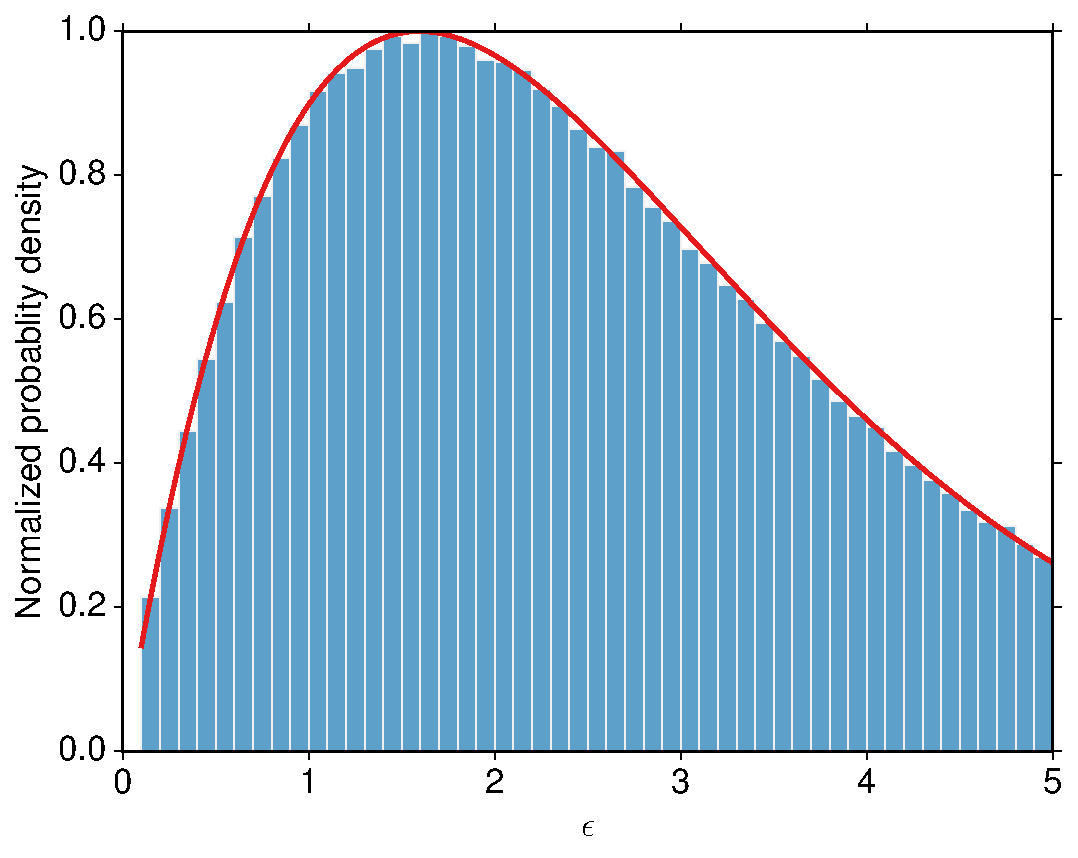
\includegraphics[width=0.8\textwidth]{bbdist.pdf}}\\
the efficiency is 67.8\%.\\
  with following code
\begin{lstlisting}[language=Python]
import numpy as np
import matplotlib.pyplot as plt

def BlackBody(epsi):
    return epsi**2/(np.exp(epsi) -1)

epsi0 = 1.59362 # result of numerical calculation

def normedBlackBody(epsi):
    """normalize the planck function so that the maximum function
    value is one"""
    return BlackBody(epsi) / BlackBody(epsi0)

e_min = 0.1
e_max = 5.0
N_photon = int(1e6)

# generate photon with random energy between e_min and e_max
photons = np.random.uniform(e_min, e_max, N_photon)

photons_BB = normedBlackBody(photons)
# second random var to judge whether reject or keep photon
randBB = np.random.uniform(0, 1, N_photon) 
photons_eff = photons[randBB <= photons_BB]

## make the plot
fig = plt.figure()
ax = fig.add_subplot(111)
hist, bins = np.histogram(photons_eff, bins=np.linspace(e_min, e_max, 50))
dbin = bins[1] - bins[0] # bin width
# matplotbar bar plot default align to the left edge
ax.bar(bins[:-1], hist/hist.max(), width=dbin, alpha=0.8)
BB_samp = np.linspace(e_min, e_max, 1000)
ax.plot(BB_samp, normedBlackBody(BB_samp), lw=2)
ax.set_xlabel('$\epsilon$')
ax.set_ylabel('Normalized probablity density') 
\end{lstlisting}
  
\bibliography{ref}
  
\end{document}